\chapter{Ανάπτυξη Διαδικτυακής Εφαρμογής iBoot}
Σε αυτό το κεφάλαιο, αναλύονται οι λειτουργίες που παρέχει η διαδικτυακή εφαρμογή στους χρήστες της μέσω Διεπαφής Χρήστη (User Interface) και παρέχεται επεξήγηση των αρχείων κώδικα, ο οποίος συντέλεσε στη δημιουργία του πληροφοριακού συστήματος. Ανάλογα με τον ρόλο του χρήστη που συνδέεται στην εφαρμογή, παρέχονται και οι αντίστοιχες λειτουργίες. Η εμφάνιση της εφαρμογής έχει ίδια αισθητικά χαρακτηριστικά για κάθε είδος χρήστη. Το User Interface θεωρείται από τα πιο σημαντικά μέρη μιας διαδικτυακής εφαρμογής καθώς, αν είναι σχεδιασμένο σωστά, ώστε να είναι εύχρηστο και διαισθητικό, κάνει εύκολη τη χρήση των λειτουργιών του συστήματος, ακόμη και σε χρήστες που πιθανώς δεν είναι εξειδικευμένοι στον τομέα της πληροφορικής.

Για την κατασκευή του User Interface, χρησιμοποιήθηκε η αρχή του Reactive Programming, δηλαδή της μεθόδου προγραμματισμού ιστού ώστε το περιεχόμενο της εφαρμογής να ανανεώνεται δυναμικά και ασύγχρονα με τις ενέργειες του χρήστη, σε ένα εν γένει στατικό περιβάλλον. Όσον αφορά το σχεδιασμό του γραφικού περιβάλλοντος, χρησιμοποιήθηκε Responsive Design, ώστε η εφαρμογή να έχει ομοιόμορφη, καλαίσθητη και λειτουργική εμφάνιση, τόσο σε συσκευές με μεγάλη διάμετρο οθόνης, όπως ηλεκτρονικούς υπολογιστές, όσο και σε συσκευές με μικρότερη διάμετρο οθόνης, όπως κινητά τηλέφωνα. Ο συνδυασμός των παραπάνω μεθόδων προγραμματισμού ιστού, προσφέρει ευχάριστη εμπειρία χρήσης της εφαρμογής, σε όλους τους χρήστες, ανεξάρτητα από τον τύπο συσκευής που χρησιμοποιούν.

Η διαδικτυακή εφαρμογή έχει υλοποιηθεί ως ένα γραφικό περιβάλλον ιστού που επικοινωνεί με τη βάση δεδομένων του μέσω ενός RESTful API. Για την ανάπτυξη της εφαρμογής έγινε χρήση του CodeIgniter PHP Framework. Η αναλυτική προδιαγραφή του API που παρέχει η πλατφόρμα, μετά την εγκατάσταση της, δημιουργήθηκε με χρήση του Swagger UI και βρίσκεται στην τοποθεσία \texttt{/api} και περιγράφει όλες τις λειτουργίες που είναι δυνατό να πραγματοποιηθούν με τη χρήση του.

\section{Διεπαφή Χρήστη}

\subsection{Εγγραφή \& Σύνδεση στο Σύστημα}

\FloatBarrier

\begin{figure}[ht]
	\centering
	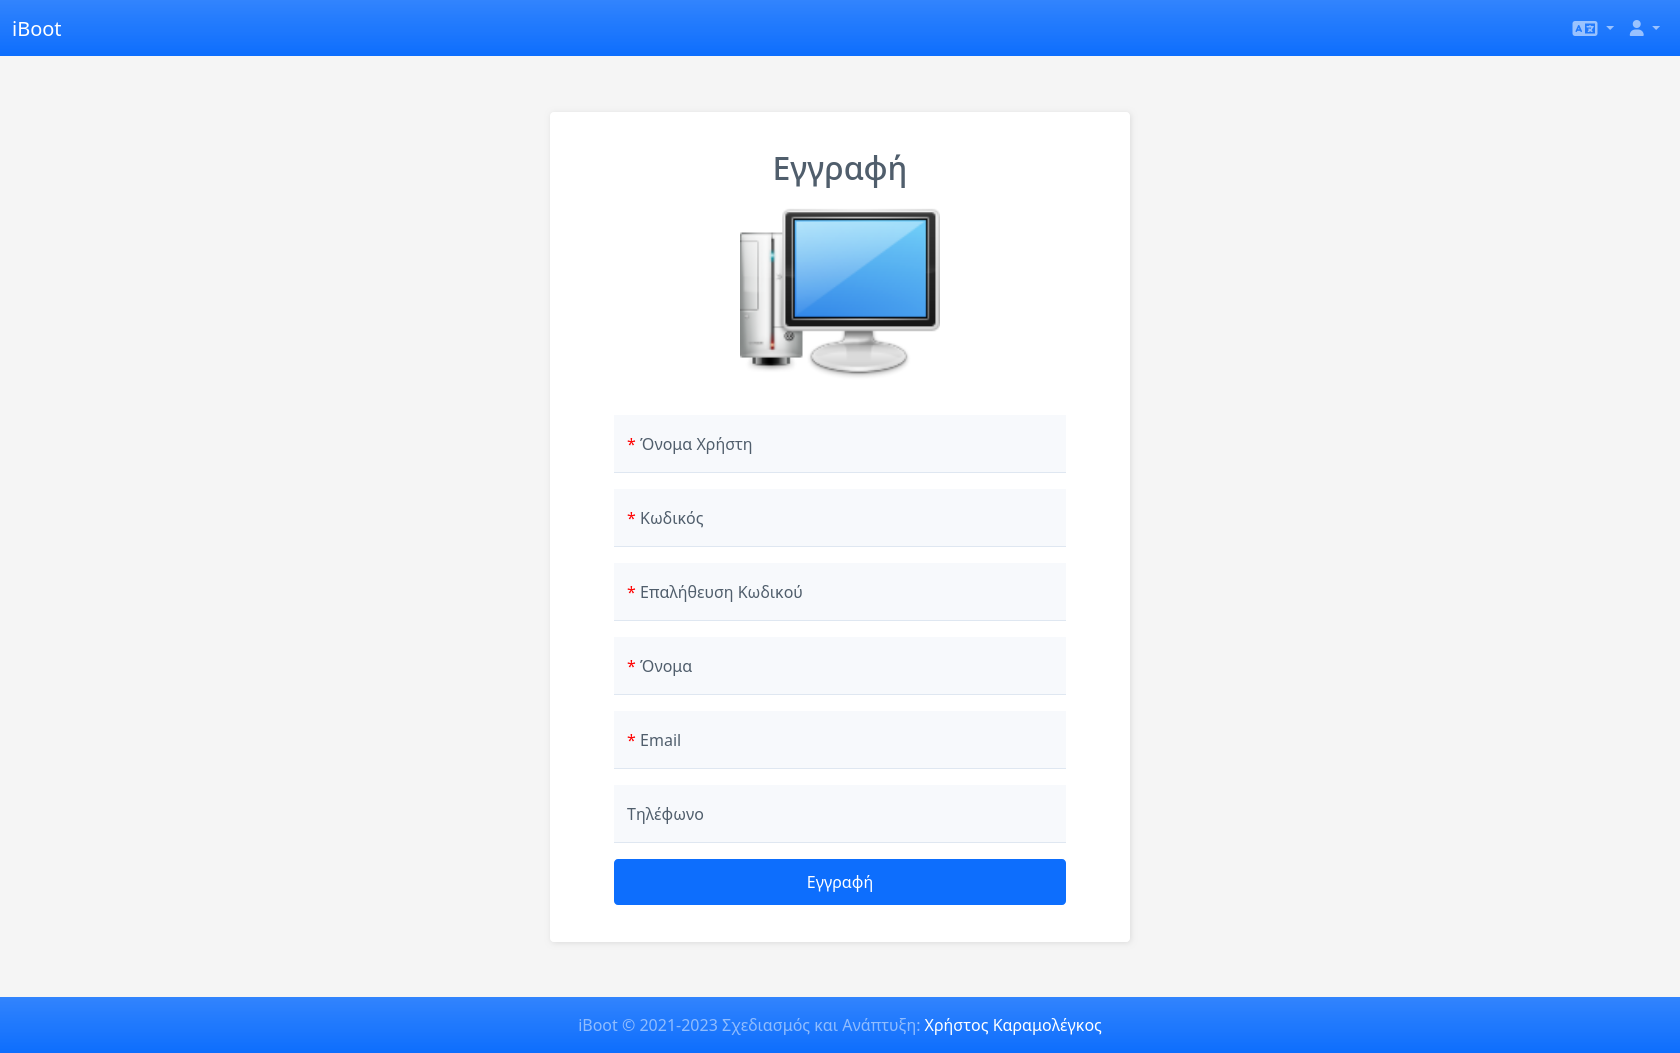
\includegraphics[scale=0.25]{iBoot-register.png}
	\caption{iBoot - Εγγραφή}
	\label{fig:iBoot_register}
\end{figure}

\begin{figure}[ht]
	\centering
	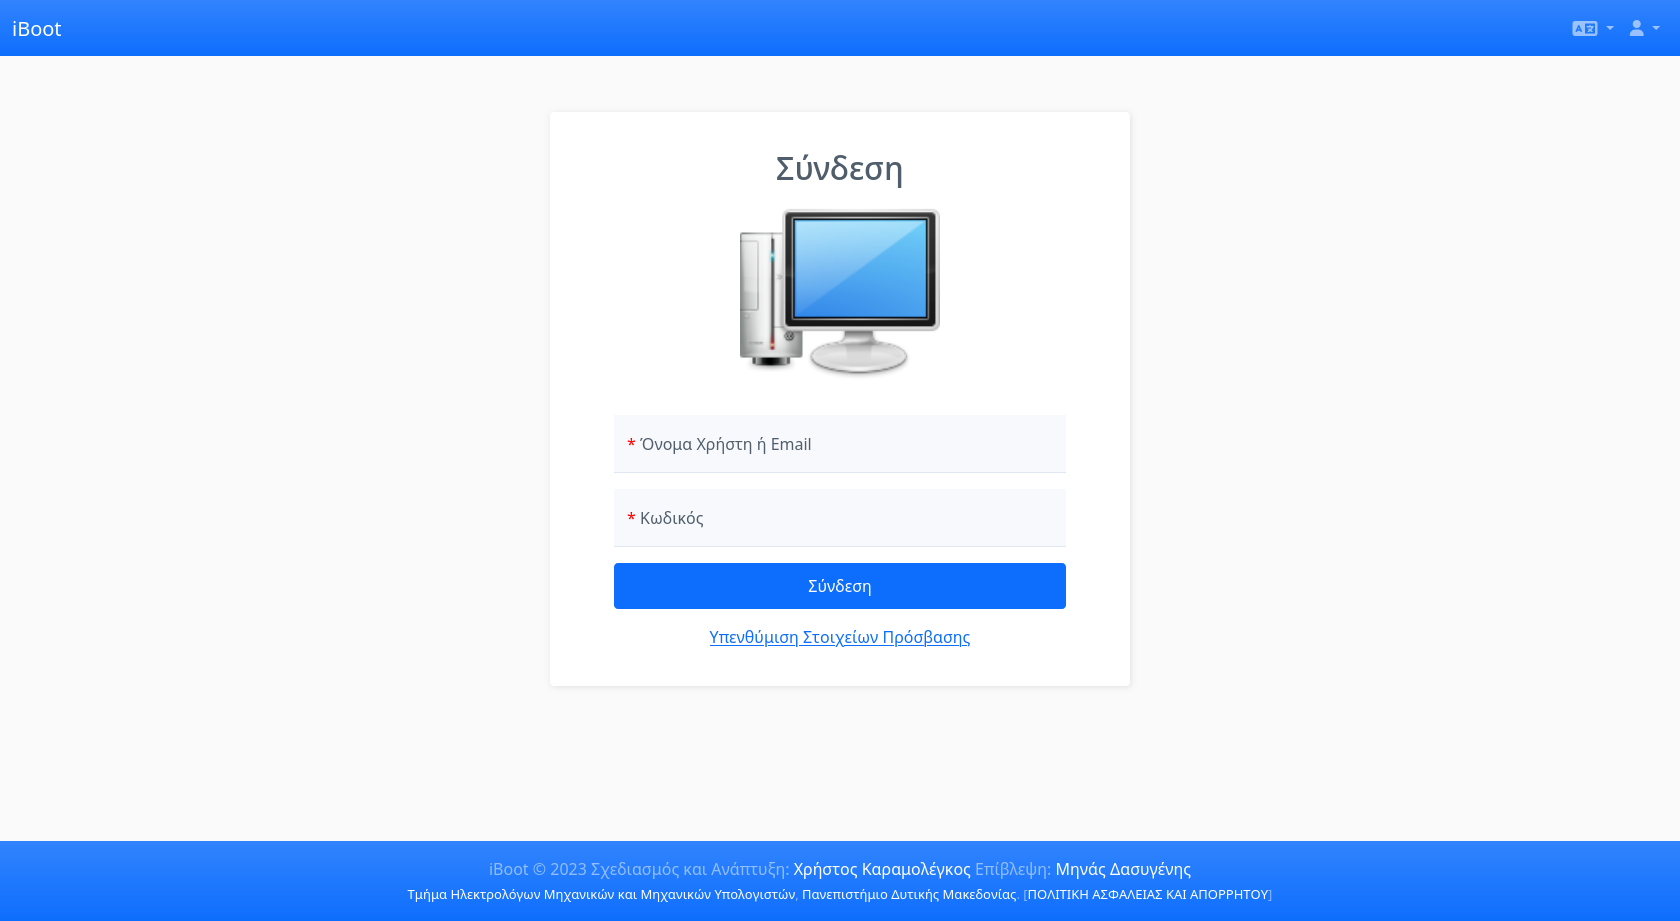
\includegraphics[scale=0.25]{iBoot-login.png}
	\caption{iBoot - Σύνδεση}
	\label{fig:iBoot_login}
\end{figure}

\begin{figure}[ht]
	\centering
	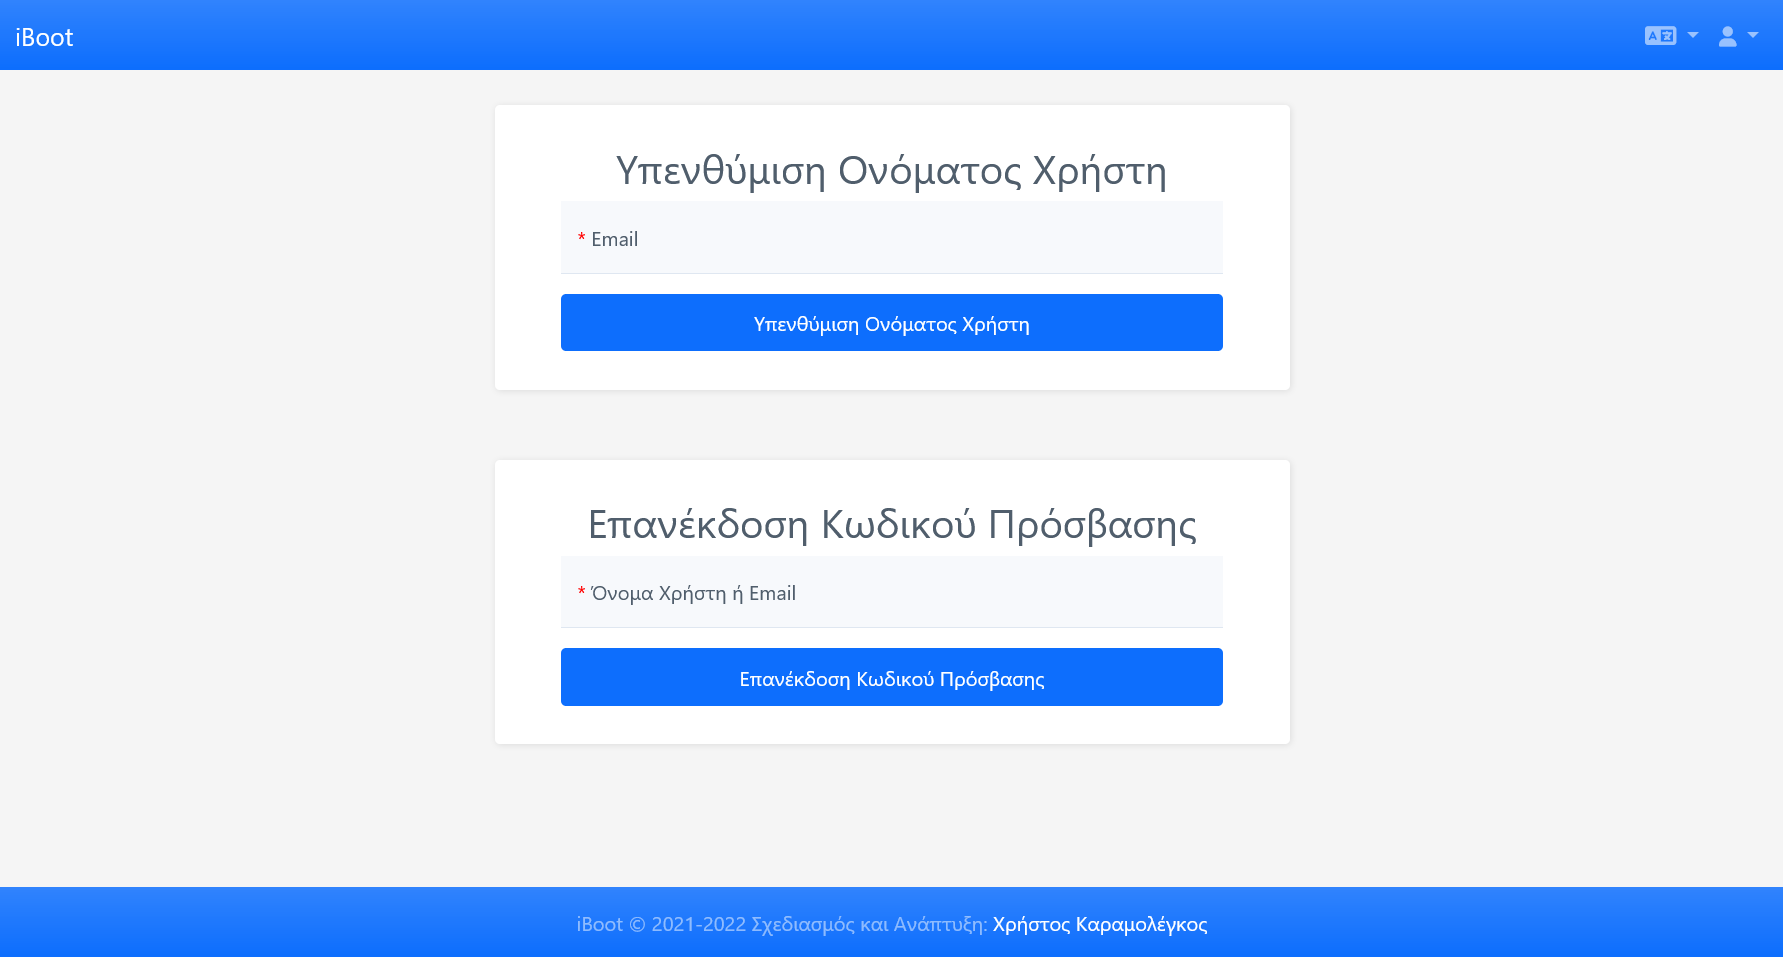
\includegraphics[scale=0.25]{iBoot-forgot-credentials.png}
	\caption{iBoot - Υπενθύμιση Στοιχείων Πρόσβασης}
	\label{fig:iBoot_forgot_credentials}
\end{figure}

\FloatBarrier

\subsection{Μενού Πλοήγησης}

\subsection{Υπολογιστές}

\subsection{Ομάδες Υπολογιστών}

\subsection{Εργαστήρια}

\subsection{Block εντολών τύπου ipxe}

\subsection{Μενού Εκκίνησης}

\subsection{Χρονοδιαγράμματα}

\subsection{Προδιαγραφή API}

\section{Επεξήγηση Αρχείων}
Καθώς η διαδικτυακή εφαρμογή αναπτύχθηκε με χρήση του CodeIgniter 4 Framework, χρησιμοποιεί και τη δομή αρχείων του \cite{CodeIgniter_structure}.

\subsection{Βασική Δομή}
Η βασική δομή της εφαρμογής αποτελείται από πέντε καταλόγους: \hyperref[ui:app]{app/}, \hyperref[ui:public]{public/}, \hyperref[ui:writable]{writable/}, \hyperref[ui:tests]{tests/} και \hyperref[ui:system]{vendor/ ή system/}.

\subsubsection{app} \label{ui:app}
Στον κατάλογο app βρίσκεται όλος ο κώδικας της εφαρμογής. Οι ακόλουθοι φάκελοι αποτελούν τα βασικά περιεχόμενα:\\

{\footnotesize
\begin{forest}
	for tree={
		font=\ttfamily,
		grow'=0,
		child anchor=west,
		parent anchor=south,
		anchor=west,
		calign=first,
		inner xsep=7pt,
		edge path={
			\noexpand\path [draw, \forestoption{edge}]
			(!u.south west) +(7.5pt,0) |- (.child anchor) pic {folder} \forestoption{edge label};
		},
		before typesetting nodes={
			if n=1
			{insert before={[,phantom]}}
			{}
		},
		fit=band,
		before computing xy={l=15pt},
	}  
	[app/
		[Config/ \ \ \ \ \ \ Αρχεία ρύθμισης παραμέτρων της εφαρμογής]
		[Controllers/ \ Οι Controllers που καθορίζουν τη ροή του προγράμματος]
		[Database/ \ \ \ \ Κλάσεις για την ενημέρωση του σχήματος και την αρχικοποίηση βάσεων δεδομένων]
		[Filters/ \ \ \ \ \ Κλάσεις φίλτρων που μπορούν να εκτελούνται πριν και μετά τους controllers]
		[Helpers/ \ \ \ \ \ Συλλογές αυτόνομων βοηθητικών συναρτήσεων]
		[Language/ \ \ \ \ Συμβολοσειρές γλώσσας για την υποστήριξη πολλαπλών γλωσσών]
		[Libraries/ \ \ \ Χρήσιμες κλάσεις που δεν ταιριάζουν σε άλλη κατηγορία]
		[Models/ \ \ \ \ \ \ Τα Models που διασυνδέουν την εφαρμογή με τη βάση δεδομένων]
		[ThirdParty/ \ \ Βιβλιοθήκες τρίτων που μπορούν να χρησιμοποιηθούν στην εφαρμογή]
		[Views/ \ \ \ \ \ \ \ Τα Views που συνθέτουν την HTML που εμφανίζεται στον πελάτη]
	]
\end{forest}
}

Στον κατάλογο app έχει δοθεί το php namespace `iBoot', έτσι ώστε τα ονόματα των αρχείων που βρίσκονται στους υποκαταλόγους του να μην συγκρούονται με ομοίως ονομαζόμενα αρχεία του Framework ή άλλων χρησιμοποιούμενων βιβλιοθηκών.

\subsubsection{public} \label{ui:public}
Ο κατάλογος public περιέχει το προσβάσιμο από το πρόγραμμα περιήγησης τμήμα της διαδικτυακής εφαρμογής, αποτρέποντας την άμεση πρόσβαση στον πηγαίο κώδικα. Περιέχει το κύριο αρχείο .htaccess, το index.php και όλα τα επιπρόσθετα στοιχεία της εφαρμογής, όπως CSS, javascript και εικόνες.

Αυτός ο φάκελος προορίζεται να είναι η "διαδικτυακή ρίζα" της εφαρμογής και ο διακομιστής ιστού θα πρέπει να ρυθμιστεί ώστε να δείχνει σε αυτόν.

\subsubsection{writable} \label{ui:writable}
Αυτός ο κατάλογος περιέχει όλους τους καταλόγους στους οποίους μπορεί να χρειαστεί να γίνει εγγραφή αρχείων κατά τη διάρκεια της ζωής της εφαρμογής. Αυτό περιλαμβάνει καταλόγους για την αποθήκευση προσωρινών αρχείων cache, αρχείων καταγραφής συμβάντων και τυχόν μεταφορτώσεις που μπορεί να στείλει ένας χρήστης. Θα πρέπει να προστεθούν εκεί όλοι οι κατάλογοι στους οποίους θα χρειαστεί να γράψει η εφαρμογή. Αυτό επιτρέπει τον ορισμό των υπόλοιπων κύριων καταλόγων ως μη εγγράψιμους, ως πρόσθετο μέτρο ασφαλείας κατά της ανεπιθύμητης τροποποίησης του κώδικα της εφαρμογής.

\subsubsection{tests} \label{ui:tests}
Αυτός ο κατάλογος έχει οριστεί για να περιέχει τα αρχεία δοκιμών. Ο κατάλογος \_support περιέχει διάφορες κλάσεις προσομοίωσης και άλλα βοηθητικά προγράμματα που μπορούν να χρησιμοποιηθούν για τη συγγραφή και εκτέλεση δοκιμών. Αυτός ο κατάλογος δεν χρειάζεται να υπάρχει στην παραγωγική εγκατάσταση της εφαρμογής.

\subsubsection{system} \label{ui:system}
Αυτός ο κατάλογος περιέχει τα αρχεία που συνθέτουν το ίδιο το CodeIgniter 4 Framework. Tα αρχεία στον κατάλογο συστήματος δεν πρέπει ποτέ να τροποποιούνται. Αντ' αυτού, μπορούν να επεκταθούν οι υπάρχουσες κλάσεις ή να δημιουργήθούν νέες, ώστε να παρέχουν την επιθυμητή λειτουργικότητα.

Όλα τα αρχεία σε αυτόν τον κατάλογο βρίσκονται κάτω από το php namespace `CodeIgniter'.

Η εγκατάσταση του framework έχει γίνει με τη βοήθεια του Composer, οπότε στην περίπτωσή μας, ο κατάλογος συστήματος βρίσκεται στη διαδρομή `vendor/codeigniter4/framework/system'.

\section{Ασφάλεια Συστήματος}
Η ασφάλεια των εφαρμογών ιστού είναι ζωτικής σημασίας επειδή οι εφαρμογές ιστού αποτελούν συχνά τον πρωταρχικό στόχο των επιτιθέμενων που επιδιώκουν να αποκτήσουν μη εξουσιοδοτημένη πρόσβαση σε ευαίσθητες πληροφορίες ή να θέσουν σε κίνδυνο τα συστήματα ενός οργανισμού. Για την διασφάλιση της ακαιρεότητας της εφαρμογής και των δεδομένων της, την προστασία της ιδιωτικότητας του κάθε χρήστη της και την εξασφάλιση της εύρυθμης και απρόσκοπτης λειτουργίας της, έχουν αξιοποιηθεί οι πρακτικές ασφαλείας που περιγράφονται παρακάτω.

\subsection{Honeypots}
Η κλάση Honeypot καθιστά δυνατό τον προσδιορισμό του πότε ένα Bot κάνει μια αίτηση στην διαδικτυακή εφαρμογή. Για να λειτουργεί, θα πρέπει να είναι ενεργοποιημένη στο αρχείο app/Config/Filters.php. Η επίτευξη της λειτουργικότητας γίνεται με την επισύναψη πεδίων εισαγωγής δεδομένων σε οποιαδήποτε φόρμα. Αυτά τα πεδία φόρμας είναι κρυμμένα από έναν άνθρωπο αλλά προσβάσιμα σε ένα Bot. Όταν εισάγονται δεδομένα στο πεδίο, θεωρείται ότι το αίτημα προέρχεται από ένα Bot και επιστρέφεται ένα HoneypotException, διακόπτοντας την εκτέλεση της αίτησης \cite{CodeIgniter_honeypots}.

\subsection{CSRF}
Η κλάση Security περιέχει μεθόδους που βοηθούν στην προστασία διαδικτυακής εφαρμογής από επιθέσεις Cross-Site Request Forgery.

Η πλαστογράφηση αιτήσεων Cross-Site Request Forgery (CSRF) είναι μια επίθεση που αναγκάζει έναν τελικό χρήστη να εκτελέσει ανεπιθύμητες ενέργειες σε μια εφαρμογή ιστού στην οποία έχει πιστοποιηθεί. Με λίγη βοήθεια κοινωνικής μηχανικής (όπως η αποστολή ενός συνδέσμου μέσω ηλεκτρονικού ταχυδρομείου ή συνομιλίας), ένας επιτιθέμενος μπορεί να εξαπατήσει τους χρήστες μιας εφαρμογής ιστού ώστε να εκτελέσουν ενέργειες της επιλογής του επιτιθέμενου. Εάν το θύμα είναι ένας κανονικός χρήστης, μια επιτυχημένη επίθεση CSRF μπορεί να αναγκάσει τον χρήστη να εκτελέσει αιτήματα αλλαγής κατάστασης, όπως μεταφορά χρημάτων, αλλαγή της διεύθυνσης ηλεκτρονικού ταχυδρομείου του κ.ο.κ. Εάν το θύμα είναι ένας διαχειριστικός λογαριασμός, το CSRF μπορεί να θέσει σε κίνδυνο ολόκληρη την εφαρμογή ιστού.

Για την πρόληψη και αντιμετώπιση των επιθέσεων CSRF υλοποιούνται οι παρακάτω μέθοδοι προστασίας και εφαρμόζονται σε όλα τα αιτήματα προς την εφαρμογή, πλην αυτών προς διευθύνσεις του REST API της.

\subsubsection{Double Submit Cookie}
Το Double Submit Cookie είναι μια τεχνική όπου στέλνουμε μια τυχαία τιμή τόσο σε ένα cookie όσο και ως παράμετρος αίτησης, με τον διακομιστή να επαληθεύει αν η τιμή του cookie και η τιμή της αίτησης ταιριάζουν. Όταν ένας χρήστης επισκέπτεται (ακόμη και πριν από την αυθεντικοποίηση για την αποτροπή του CSRF σύνδεσης), ο ιστότοπος παράγει μια κρυπτογραφικά ισχυρή τυχαία τιμή και τη θέτει ως cookie στον υπολογιστή του χρήστη ξεχωριστά από το αναγνωριστικό συνεδρίας. Στη συνέχεια, ο ιστότοπος απαιτεί κάθε αίτημα συναλλαγής να περιλαμβάνει αυτή την τυχαία τιμή ως κρυφή τιμή φόρμας ή στην επικεφαλίδα του αιτήματος. Εάν και οι δύο ταιριάζουν στην πλευρά του διακομιστή, ο διακομιστής το δέχεται ως νόμιμο αίτημα, ενώ εάν δεν ταιριάζουν, θα απορρίψει το αίτημα.

Με λίγα λόγια, ένας εισβολέας δεν μπορεί να έχει πρόσβαση στην τιμή του cookie κατά τη διάρκεια ενός cross-site αιτήματος. Αυτό τους εμποδίζει να συμπεριλάβουν μια τιμή που ταιριάζει στην κρυφή τιμή της φόρμας ή ως παράμετρος/κεφαλίδα αίτησης.

\subsubsection{Τυχαιοποίηση token}
Για να μετριαστούν οι επιθέσεις πλευρικού καναλιού συμπίεσης όπως το BREACH και να αποτραπεί η προσπάθεια ενός εισβολέα από το να μαντέψει τα διακριτικά CSRF, είναι ενεργοποιημένη η τυχαιοποίηση των διακριτικών. Έτσι, μια τυχαία μάσκα προστίθεται στο κάθε token και χρησιμοποιείται για την κρυπτογράφησή του.

\subsubsection{Αναγέννηση Token}
Τα tokens αναδημιουργούνται σε κάθε υποβολή του CSRF cookie. Η αναγέννηση των tokens παρέχει αυστηρότερη ασφάλεια, αλλά μπορεί να οδηγήσει σε μειωμένη ευχρηστία, καθώς άλλα tokens που καθίστανται άκυρα μπορεί να χρειαστεί να χρησιμοποιηθούν εκ νέου σε περιπτώσεις όπως πλοήγηση προς τα πίσω/εμπρός, πολλαπλές καρτέλες/παράθυρα, ασύγχρονες ενέργειες κ.λπ. Το παραπάνω αρνητικό δε θεωρείται μεγάλης σημαντικότητας σε σχέση με την αυξημένη ασφάλεια που προσφέρει το μέτρο της αναγέννησης των tokens.

\subsection{JWT}
Η αυθεντικοποίηση στο REST API της εφαρμογής, έχει υλοποιηθεί με χρήση JSON Web Tokens (JWT).

\subsubsection{Λειτουργία JWT}
Αρχικά, ο χρήστης ή η εφαρμογή-πελάτης στέλνει ένα αίτημα σύνδεσης. Σε αυτό το βήμα, ουσιαστικά, ένα όνομα χρήστη, ένας κωδικός πρόσβασης ή οποιοσδήποτε άλλος τύπος διαπιστευτηρίων σύνδεσης που παρέχει ο χρήστης θα ταξιδέψει στο API. Μόλις επαληθευτεί, το API θα δημιουργήσει ένα JSON Web Token και θα το υπογράψει χρησιμοποιώντας ένα μυστικό κλειδί. Στη συνέχεια, το API θα επιστρέψει αυτό το token πίσω στην εφαρμογή-πελάτη.

Τέλος, η εφαρμογή-πελάτης θα λάβει το token, θα το επαληθεύσει στη δική της πλευρά για να διασφαλίσει ότι είναι αυθεντικό και στη συνέχεια θα το χρησιμοποιήσει σε κάθε επόμενη αίτηση. Ως εκ τούτου, μπορεί να πιστοποιήσει τον χρήστη χωρίς να χρειάζεται να στείλει πλέον τα διαπιστευτήριά του.

Η διαδικασία έκδοσης και χρήσης JWT token απεικονίζεται στο σχήμα \ref{fig:JWT_authentication}.

\begin{figure}[h]
	\centering
	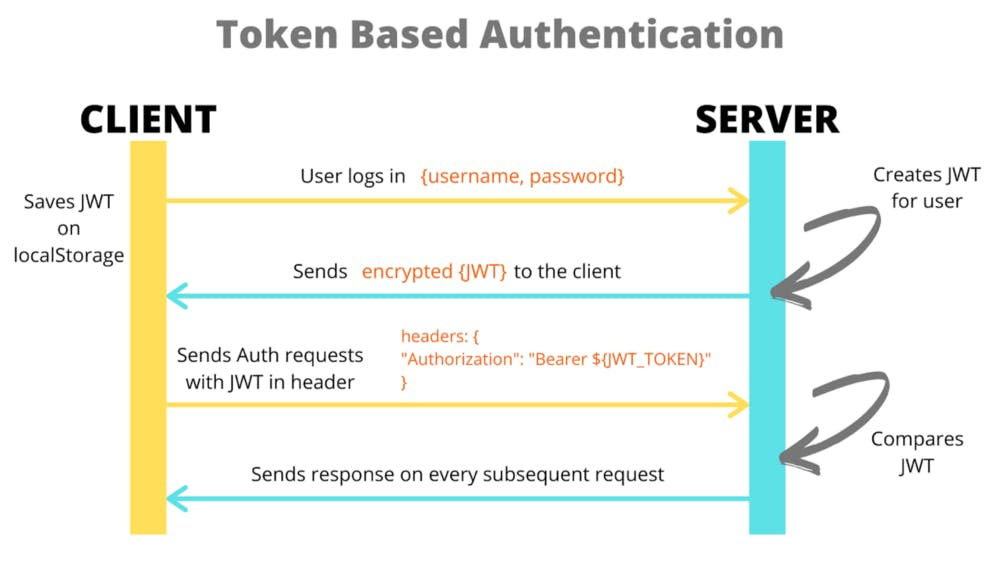
\includegraphics[scale=0.4]{JWT_authentication.jpg}
	\caption[{Λειτουργία JWT}]{Λειτουργία JWT \textbf{Πηγή:} \cite{fig_JWT_authentication}}
	\label{fig:JWT_authentication}
\end{figure}

\subsubsection{Δομή JWT}
Το ίδιο το token, το οποίο επιστρέφεται από το API, είναι απλώς μια κωδικοποιημένη συμβολοσειρά. Αποτελείται από τρία διαφορετικά τμήματα, τα οποία διαχωρίζονται μεταξύ τους με έναν χαρακτήρα τελείας. Αυτά είναι το header, το payload και το signature.

To header περιέχει δεδομένα σχετικά με τον τύπο του κουπονιού και τον αλγόριθμο που χρησιμοποιείται για τη δημιουργία του.

Το payload περιέχει δεδομένα σχετικά με την αίτηση και τον χρήστη που την υπέβαλε. Υπάρχει ένα σύνολο τυποποιημένων ζευγών κλειδιών/τιμών που ορίζονται ως μέρος του JWT, τα οποία μπορούν να χρησιμοποιηθούν:
\begin{itemize}
  \item Sub (Subject): Προσδιορίζει τον χρήστη που κάνει την αίτηση και πιστοποιείται.
  \item Iss (Issuer): Ο διακομιστής που εξέδωσε το token. Στην περίπτωσή μας, θα είχε νόημα να συμπεριλάβουμε το URI που χρησιμοποιείται
  \item Aud (Audience): Παρέχει κάποια μορφή ταυτοποίησης του παραλήπτη αυτού του κουπονιού.
  \item Exp (Ημερομηνία λήξης): Τα κουπόνια συνήθως δεν διαρκούν για πάντα. Η Exp εξασφαλίζει ότι όποιος χρησιμοποιεί το token παρέχει ένα πρόσφατα δημιουργημένο token.
\end{itemize}
Επίσης, είναι δυνατόν να καθοριστούν επιπρόσθετα ζεύγη κλειδιών/τιμών για την κάλυψη των αναγκών της υλοποίησης.

Τέλος, το signature είναι απλώς μια κωδικοποιημένη συμβολοσειρά που χρησιμοποιείται τόσο από τον διακομιστή όσο και από τον πελάτη για την επαλήθευση της αυθεντικότητας του payload.

Η αποκωδικοποιημένη δομή ενός παραδείγματος JWT token απεικονίζεται στο σχήμα \ref{fig:JWT_structure}.

\begin{figure}[h]
	\centering
	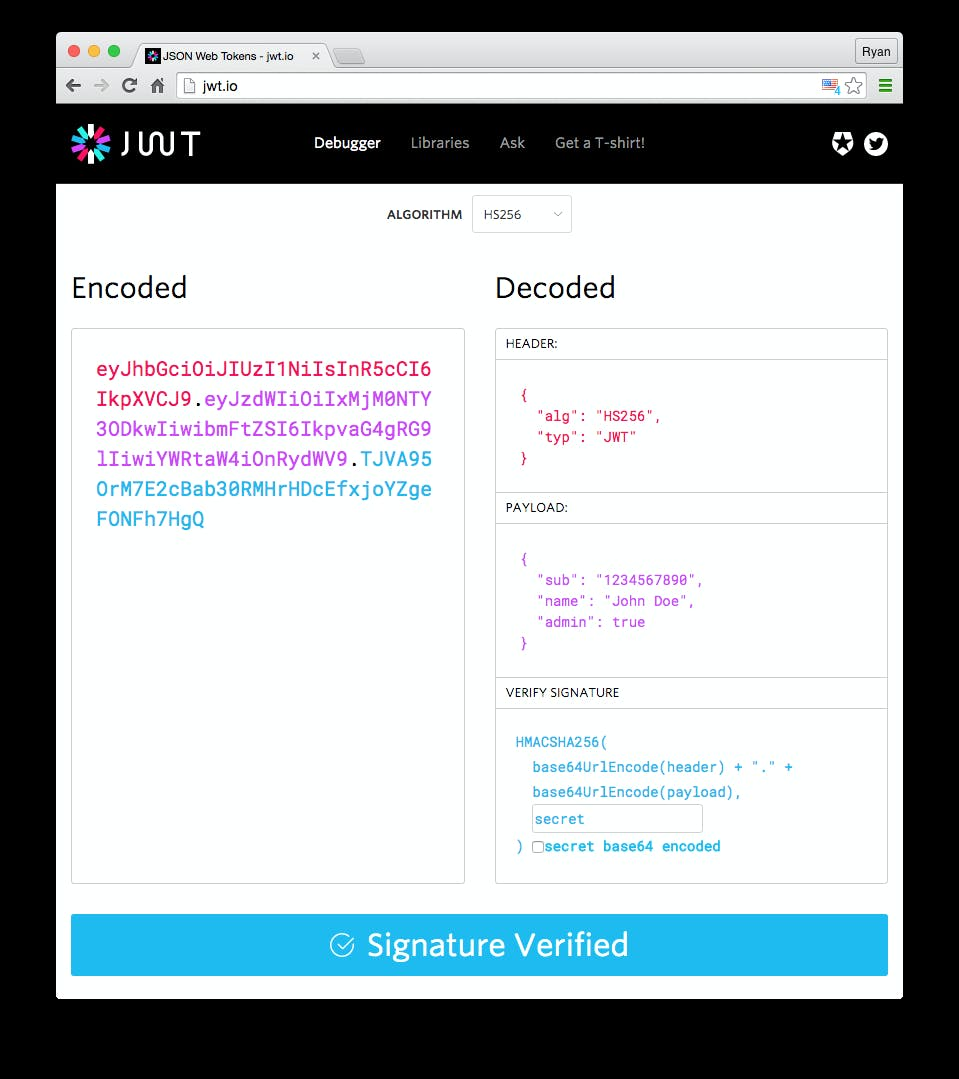
\includegraphics[scale=0.4]{JWT_structure.jpg}
	\caption[{Δομή JWT}]{Δομή JWT \textbf{Πηγή:} \cite{fig_JWT_structure}}
	\label{fig:JWT_structure}
\end{figure}

\subsection{Αντιμετώπιση SQL Injections}
\subsubsection{Τι είναι SQL Injection;}
Οι επιθέσεις τύπου SQL Injection προσπαθούν να εκμεταλλευτούν μια ευπάθεια στην ασφάλεια μιας διαδικτυακής εφαρμογής, η οποία επιτρέπει σε έναν εισβολέα να παρεμβαίνει στα ερωτήματα που κάνει η εφαρμογή στη βάση δεδομένων της. Αν υπάρχει ευπάθεια και ο εισβολέας καταφέρει να την εκμεταλλευτεί, μπορεί να αποκτήσει πρόσβαση σε δεδομένα που κανονικά δεν θα έπρεπε να είναι σε θέση να ανακτήσει ή ακόμη και να προκαλέσει καταστροφή της βάσης και απώλεια δεδομένων. Η αντιμετώπιση τέτοιων ευπαθειών είναι μείζονος σημασίας στις διαδικτυακές εφαρμογές, αφού οι επιθέσεις SQL Injection αποτελούν έναν από τους πιο διαδεδομένους τρόπους επίθεσης, είτε από μόνες τους, είτε σε συνδυασμό με άλλου τύπου επιθέσεις όπως DDoS attacks, DNS hijacking και Cross-Site Scripting (XSS).

\subsubsection{Prepared SQL Statements}
Οι προμεταγλωττισμένες εντολές SQL βοηθούν στην αντιμετώπιση των επιθέσεων τύπου SQL Injection. Με τη χρήση προμεταγλωττισμένων εντολών, οι τιμές των μεταβλητών που λαμβάνονται από τον χρήστη, αφού περάσουν από φίλτρο αντικατάστασης χαρακτήρων με ειδική σημασία στην SQL, ενσωματώνονται στην προμεταγλωττισμένη εντολή για να συνθέσουν το τελικό query που θα εκτελεστεί στη βάση δεδομένων. Έτσι, ενδεχόμενες κακόβουλες υποβολές τιμών από χρήστες, δε φτάνουν στο να εκτελεστούν στη βάση δεδομένων και να προκαλέσουν απώλεια ή υποκλοπή πληροφοριών.

\subsubsection{Ληφθέντα μέτρα αντιμετώπισης SQL Injections}
Η κλάση Query Builder του CodeIgniter4 \cite{CodeIgniter_querybuilder} έχει χρησιμοποιηθεί για την επικοινωνία της εφαρμογής με τη βάση δεδομένων της. Οι συναρτήσεις, που παρέχονται από τη συγκεκριμένη κλάση, καλούνται διαδοχικά και κάθε μια, με την εκτέλεσή της, προσθέτει από μια παράμετρο ώστε να συντεθεί το τελικό SQL Query προς εκτέλεση. Δέχονται ως ορίσματα τις απαραίτητες μεταβλητές, στις οποίες πραγματοποιούν αυτόματα την αντικατάσταση των ειδικών χαρακτήρων. Όταν κληθεί μια συνάρτησης ανάκτησης πληροφορίας από τη βάση, οι μεταβλητές ενσωματώνονται στο prepared query που έχει συνθέσει η κλήση των προηγούμενων συναρτήσεων, το ερώτημα εκτελείται και επιστρέφεται το αποτέλεσμα.

Για επιπρόσθετη ασφάλεια, καθώς η αντικατάσταση ειδικών χαρακτήρων δεν επαρκεί από μόνη της, αλλά και για κανονικοποίηση και επαλήθευση των τιμών των μεταβλητών του κάθε Μοντέλου, πριν ακόμη αυτές εισαχθούν στη βάση δεδομένων, έχει χρησιμοποιηθεί επίσης η βιβλιοθήκη Validation \cite{CodeIgniter_validation}. Στο κάθε Μοντέλο διατηρείται ένας πίνακας, ο οποίος περιέχει τα απαραίτητα φίλτρα επαλήθευσης για την κάθε τιμή μεταβλητής που δόθηκε από τον χρήστη ως είσοδος. Ο έλεγχος πραγματοποιείται πριν την εισαγωγή των δεδομένων στη βάση, η οποία πραγματοποιείται μόνο αν επικυρωθεί ότι οι τιμές που εξετάζονται είναι στη σωστή μορφή και τύπο.

Για παράδειγμα, έχει οριστεί ότι το αναγνωριστικό (ID) κάθε γραμμής ενός πίνακα, είναι ένας θετικός ακέραιος αριθμός. Αν ο χρήστης δοκιμάσει να εισάγει ως αναγνωριστικό κάποια είσοδο που δεν ικανοποιεί τον παραπάνω κανόνα, όπως κάποιο χαρακτήρα, η είσοδος θα απορριφθεί κατά τον έλεγχο εγκυρότητάς της. Ομοίως, δε θα γίνει αποδεκτή η είσοδος, αν στο πεδίο του email δεν είναι έγκυρο email ή αν το email που δόθηκε υπάρχει ήδη στον πίνακα, αφού έχει οριστεί και ως μοναδικό.

Ο συνδυασμός των παραπάνω πρακτικών, δηλαδή του ελέγχου εγκυρότητας των εισόδων και της ενσωμάτωσής τους σε prepared SQL statements, αποτελεί μια πολύ ισχυρή άμυνα ενάντια σε επιθέσεις τύπου SQL Injection.

\section{Σύνοψη Κεφαλαίου 4}
Στο κεφάλαιο 4, εξετάστηκαν όλες οι δυνατότητες της διαδικτυακής εφαρμογής και τα βήματα που πρέπει να ακολουθήσει ένας νέος χρήστης για να τις χρησιμοποιήσει. Επιπλέον, παρασχέθηκε οπτικό υλικό για κάθε λειτουργία στην οποία εμφανιζόταν στον χρήστη η διεπαφή χρήστη της διαδικτυακής εφαρμογής κατά την πλοήγησή του. Στη συνέχεια, εξηγήθηκαν διεξοδικά τόσο το front-end όσο και το back-end της δομής του πληροφοριακού συστήματος. Προκειμένου να διασφαλιστεί η ασφάλεια κατά τη χρήση της διαδικτυακής εφαρμογής, παρέχεται επεξήγηση των πρωτοκόλλων και των προσεγγίσεων ασφαλείας.

Στο επόμενο κεφάλαιο θα γίνει αξιολόγηση του συστήματος, ως προς την ορθή λειτουργία του και τις δυνατότητες κλιμάκωσής του.
